\let\negmedspace\undefined
\let\negthickspace\undefined
\documentclass[journal]{IEEEtran}
\usepackage[a5paper, margin=10mm, onecolumn]{geometry}
%\usepackage{lmodern} % Ensure lmodern is loaded for pdflatex
\usepackage{tfrupee} % Include tfrupee package

\setlength{\headheight}{1cm} % Set the height of the header box
\setlength{\headsep}{0mm}     % Set the distance between the header box and the top of the text

\usepackage{gvv-book}
\usepackage{gvv}
\usepackage{cite}
\usepackage{amsmath,amssymb,amsfonts,amsthm}
\usepackage{algorithmic}
\usepackage{graphicx}
\usepackage{textcomp}
\usepackage{xcolor}
\usepackage{txfonts}
\usepackage{listings}
\usepackage{enumitem}
\usepackage{mathtools}
\usepackage{gensymb}
\usepackage{comment}
\usepackage[breaklinks=true]{hyperref}
\usepackage{tkz-euclide} 
\usepackage{listings}
% \usepackage{gvv}                                        
\def\inputGnumericTable{}                                 
\usepackage[latin1]{inputenc}                                
\usepackage{color}                                            
\usepackage{array}                                            
\usepackage{longtable}                                       
\usepackage{calc}                                             
\usepackage{multirow}                                         
\usepackage{hhline}                                           
\usepackage{ifthen}                                           
\usepackage{lscape}
\usepackage{circuitikz}
\tikzstyle{block} = [rectangle, draw, fill=blue!20, 
    text width=4em, text centered, rounded corners, minimum height=3em]
\tikzstyle{sum} = [draw, fill=blue!10, circle, minimum size=1cm, node distance=1.5cm]
\tikzstyle{input} = [coordinate]
\tikzstyle{output} = [coordinate]


\begin{document}

\bibliographystyle{IEEEtran}
\vspace{3cm}

\title{1.2.24}
\author{AI25BTECH11016-Varun}
 \maketitle
% \newpage
% \bigskip
{\let\newpage\relax\maketitle}
\renewcommand{\thefigure}{\theenumi}
\renewcommand{\thetable}{\theenumi}
\setlength{\intextsep}{10pt} % Space between text and floats
\numberwithin{figure}{enumi}
\renewcommand{\thetable}{\theenumi}
\textbf{Question}:\\

Rain is falling vertically with a speed of 35 m/s. Wind starts blowing after some time with a speed of 12 m/s in the east to west direction. In which direction should a boy waiting at a bus stop hold his umbrella?\\

\solution \\

$\vec{v}_{r/w}$ be the velocity of rain relative to the wind (downward), 


$\vec{v}_{r/w}$ = \myvec{0 \\ -35}

$\vec{v}_{w}$ be the velocity of wind relative to ground

$\vec{v}_w $= \myvec{-12 \\ 0}

$\vec{v}_{r}$ be the velocity of rain relative to ground 
Take $+x$ to the east and $+y$ upward.


\textbf{Resultant rain velocity (relative to ground).}
\begin{align}
    \vec{v}_{r} &= \vec{v}_{w} + \vec{v}_{r/w}
\end{align}


\textbf{Angle from vertical (downward).} Let $\theta$ be the angle between $\vec{v}_{r}$ and the downward vertical unit vector $$\hat{u}_{\downarrow}=\begin{myvec}{0\\-1}\end{myvec}$$.




Using the dot product,
\begin{align}
    \cos\theta &= \frac{\vec{v}_{r}\cdot \hat{u}_{\downarrow}}{\|\vec{v}_{r}\|} \\
    \cos\theta &= \frac{v_{r/w}}{\sqrt{v_{r/w}^2 + v_w^2}}
\end{align}
\text{Equation 3 is obtained by substituting Equation 1 in Equation 2 }



Substitute given values.

For this problem, the speed of rain w.r.t wind is $v_{r/w}=35\ \text{m/s}$ 

the wind speed is $v_w=12\ \text{m/s}$ (east to west).
\begin{align}
    \cos\theta &= \frac{35}{\sqrt{35^2 + 12^2}} \\
    \cos\theta &= \frac{35}{37} \\ 
        \theta &= \cos^{-1}\!\left(\frac{35}{37}\right)
\end{align}



Rain falls at an angle of 
$\theta=\cos^{-1}\!\left(\frac{35}{37}\right)$ west of vertical downward

The rain's velocity component is toward the west and downward, so the umbrella must be kept in the opposite direction:

Hence,
\begin{align}
 \text{Umbrella direction should be at an angle} \cos^{-1}\!\left(\frac{35}{37}\right)\ \text{east of vertical upward.} \nonumber
\end{align}


\begin{figure}[h]
    \centering
    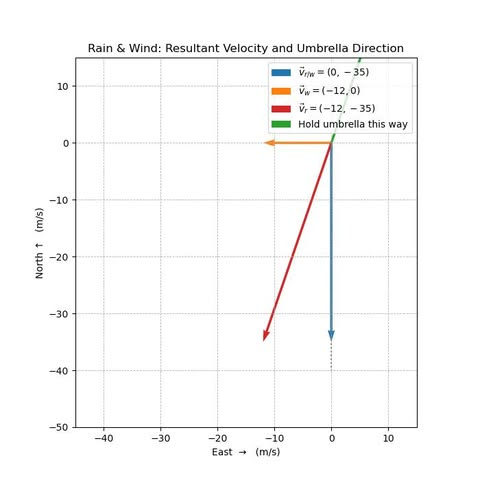
\includegraphics[scale=0.5]{figs/1.2.24.jpg}
    \caption{}
    \label{fig:1}
\end{figure}

\end{document}